\documentclass[10pt]{article}
%%%%%%%%%%%%%%%%%%%%%%%%%
%			AZ' STANDARD NEWCOMMANDS
%%%%%%%%%%%%%%%%%%%%%%%%%
\usepackage[applemac]{inputenc}
\usepackage[english]{babel}
\usepackage[T1]{fontenc}
\usepackage{cite, url,color} % Citation numbers being automatically sorted and properly "compressed/ranged".
%\usepackage{pgfplots}
\usepackage{graphics,amsfonts}
\usepackage[pdftex]{graphicx}
\usepackage[cmex10]{amsmath}
% Also, note that the amsmath package sets \interdisplaylinepenalty to 10000
% thus preventing page breaks from occurring within multiline equations. Use:
 \interdisplaylinepenalty=2500
% after loading amsmath to restore such page breaks as IEEEtran.cls normally does.

%% Useful packages for creation of two-column and more complex figures
% Compact lists
\usepackage{enumitem}
\usepackage{booktabs}
\usepackage{fancyvrb}

\usepackage{listings} % inserisce listati di programmi
\definecolor{commenti}{rgb}{0.13,0.55,0.13}
\definecolor{stringhe}{rgb}{0.63,0.125,0.94}
\lstloadlanguages{Matlab}
\lstset{% general command to set parameter(s)
framexleftmargin=0mm,
frame=single,
keywordstyle = \color{blue},% blue keywords
identifierstyle =, % nothing happens
commentstyle = \color{commenti}, % comments
stringstyle = \ttfamily \color{stringhe}, % typewriter type for strings
showstringspaces = false, % no special string spaces
emph = {for, if, then, else, end},
emphstyle = \color{blue},
firstnumber = 1, % numero della prima linea
numbers =right, %  show number_line
numberstyle = \tiny, % style of number_line
stepnumber = 5, % one number_line after stepnumber
numbersep = 5pt,
language = {Matlab}, % per riconoscere la sintassi matlab
extendedchars = true, % per abilitare caratteri particolari
breaklines = true, % per mandare a capo le righe troppo lunghe
breakautoindent = true, % indenta le righe spezzate
breakindent = 30pt, % indenta le righe di 30pt
basicstyle=\footnotesize\ttfamily
}

\usepackage{array}
% http://www.ctan.org/tex-archive/macros/latex/required/tools/
\usepackage{mdwmath}
\usepackage{mdwtab}
%mdwtab.sty	-- A complete ground-up rewrite of LaTeX's `tabular' and  `array' environments.  Has lots of advantages over
%		   the standard version, and over the version in `array.sty'.
% *** SUBFIGURE PACKAGES ***
\usepackage[tight,footnotesize]{subfigure}

\usepackage[top=2cm, bottom=2cm, right=1.6cm,left=1.6cm]{geometry}
\usepackage{indentfirst}

%\usepackage{times}
%\usepackage[active]{srcltx}
\graphicspath{{./figure/}}

\setlength\parindent{0pt}
\linespread{1}

\def\C#1{\mathcal{#1}}

\usepackage{mathtools}
\DeclarePairedDelimiter{\ceil}{\lceil}{\rceil}
\DeclarePairedDelimiter{\floor}{\lfloor}{\rfloor}

% Package used to keep inherent figures in the same section
\usepackage{placeins}


\begin{document}
\title{Network Analysis and Simulation - Homework 2}
\author{Michele Polese, 1100877}

\maketitle

\section{Exercise 1}
Figure~\ref{fig:65} shows the randomness of a U[0,1] sequence generated with a \textit{Linear Congruential Generator} (LCG) in different ways: by comparing with a U[0, 1] generated by MATLAB Mersenne Twister rng, by showing the lac of correlation between samples with the autocorrelation function and lag plots.
\begin{figure}
  \centering
  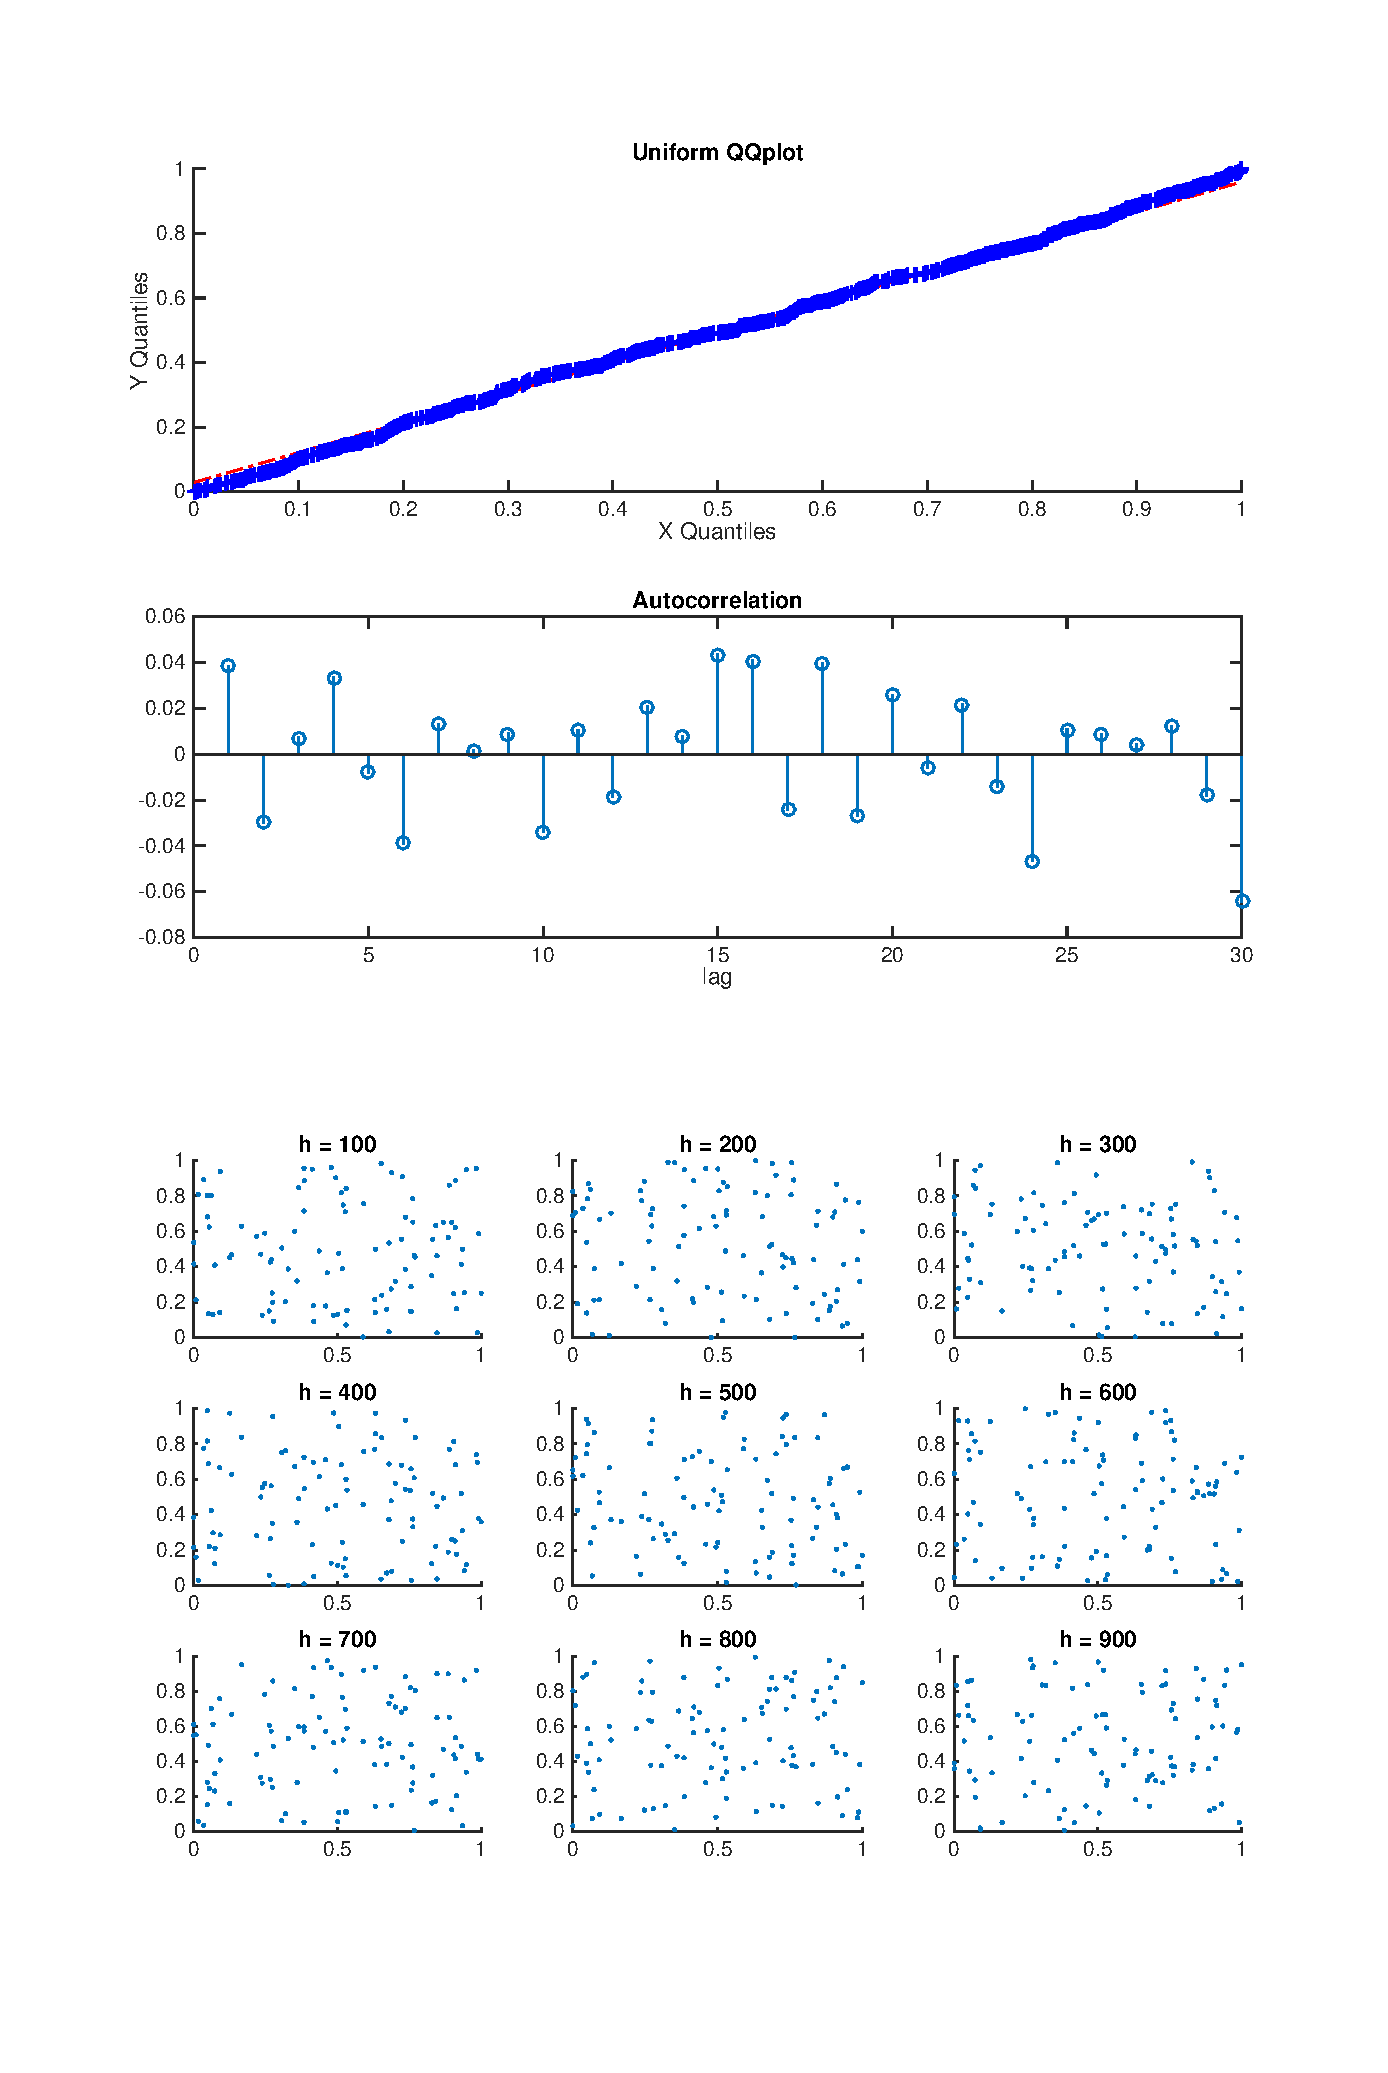
\includegraphics[width=0.7\textwidth]{images/hw2_1_65}
  \caption{Figure 6.5 in \cite{leb}}
  \label{fig:65}
\end{figure}

Figure~\ref{fig:67} shows that a LCG must be handled carefully when dealing with parallel streams. Indeed
\begin{figure}
  \centering
  \subfigure{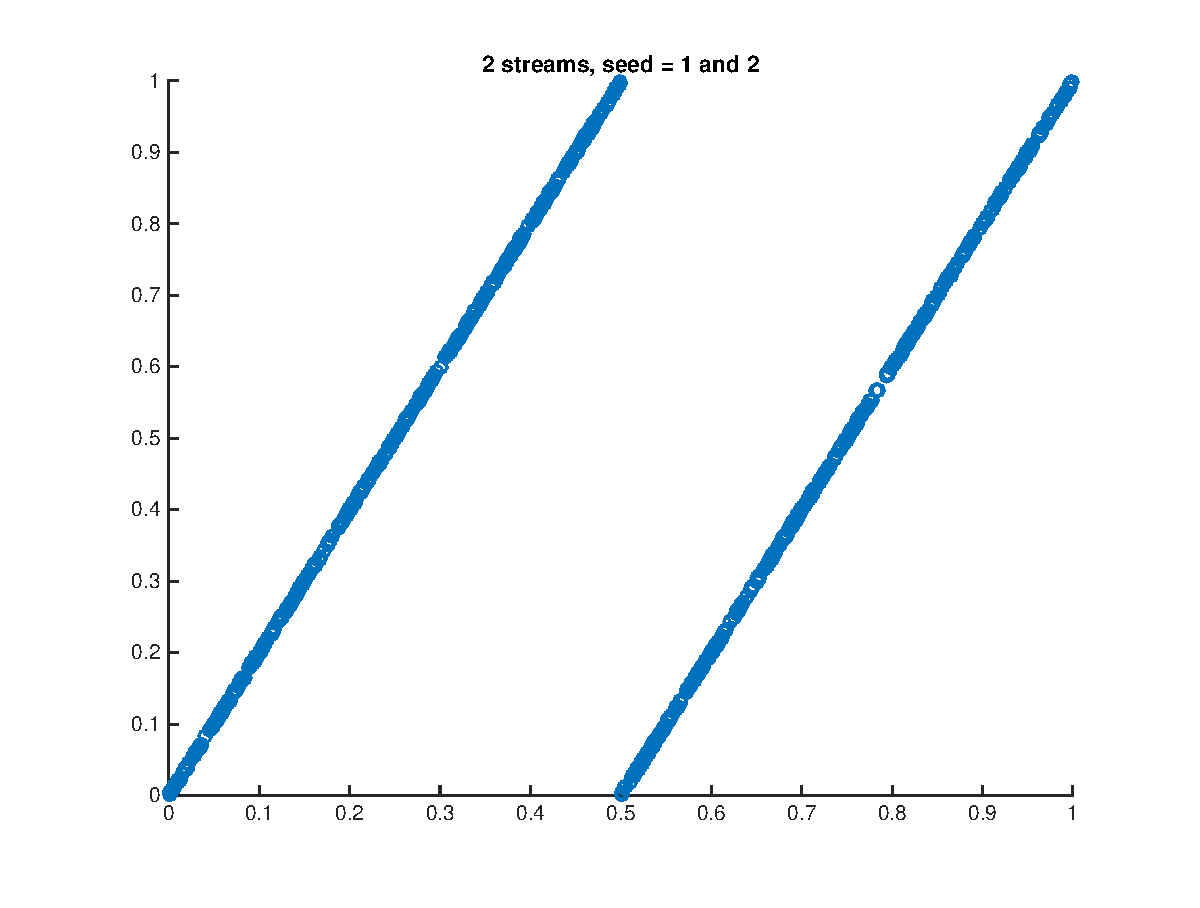
\includegraphics[width=0.7\textwidth]{images/hw2_1_67a}}
  \subfigure{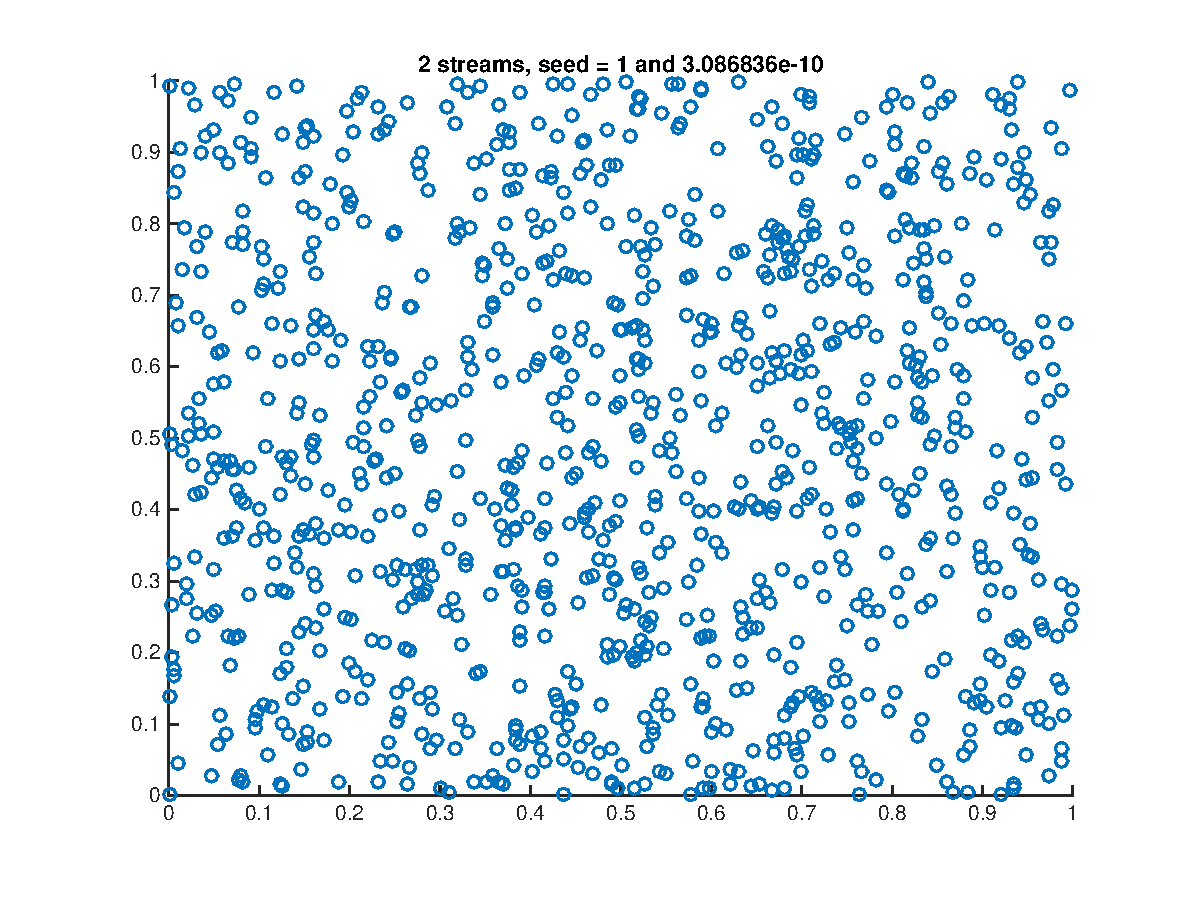
\includegraphics[width=0.7\textwidth]{images/hw2_1_67b}}
  \caption{Figure 6.7 in \cite{leb}}
  \label{fig:67}
\end{figure}

\begin{figure}
  \centering
  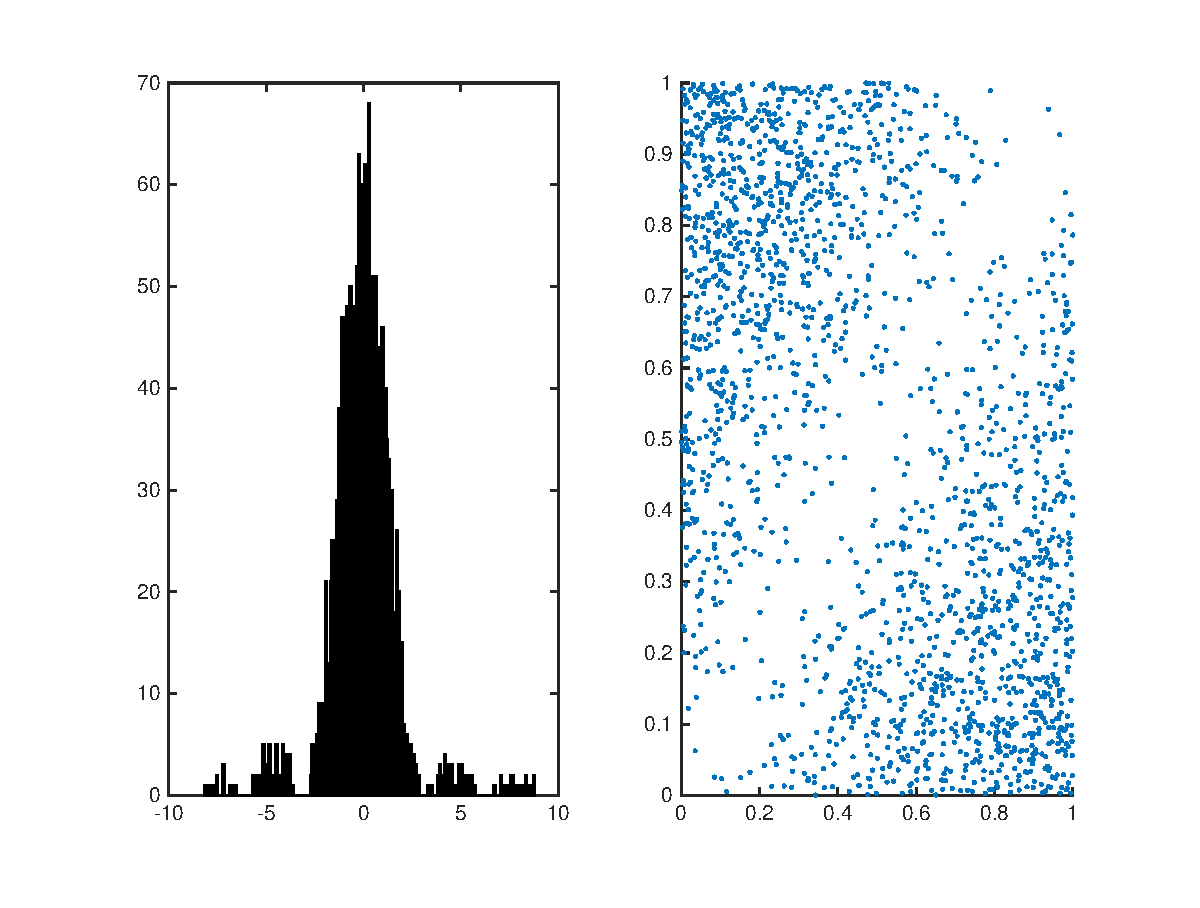
\includegraphics[width=0.7\textwidth]{images/hw2_1_610}
  \caption{Figure 6.10 in \cite{leb}}
  \label{fig:610}
\end{figure}

\begin{thebibliography}{10}

\bibitem{leb}
Y. Le Boudec, Performance Evaluation of Computer and Communications Systems, EPFL, 2015

\bibitem{pk}
M. Pinsky, S. Karlin, An Introduction to Stochastic Modeling, $4^{th}$ edition, Elsevier, 2011


\end{thebibliography}

\end{document}
